\pdfminorversion=4

\documentclass[varwidth=true,11pt]{standalone}

\usepackage{amsmath}
\usepackage[T1]{fontenc}
\usepackage{lmodern}
\usepackage{tikz}

\begin{document}
\thispagestyle{empty}

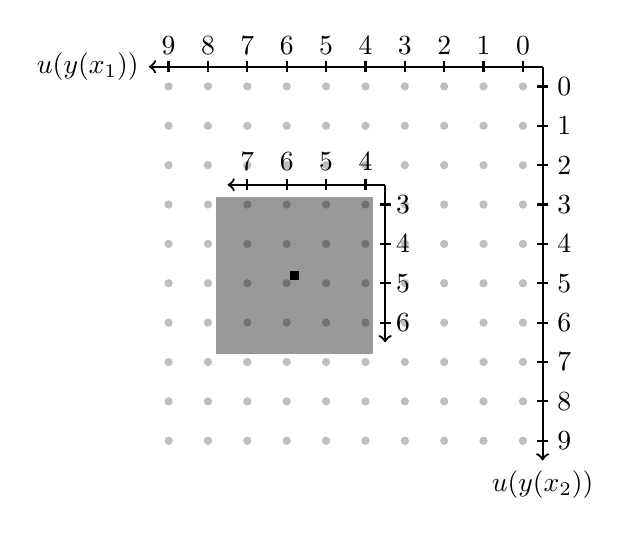
\begin{tikzpicture}[baseline=(current bounding box.center),scale=0.5]
% draw coordinate axes
\draw[thick] [->](9.5,9.5) -- (-0.5,9.5) node[left]{$u(y(x_1))$};
\draw[thick] [->](9.5,9.5) -- (9.5,-0.5) node[anchor=north]{$u(y(x_2))$};
% draw labels
\foreach \x in {0,...,9} {\draw[thick] (9-\x,9.5cm+4pt) -- (9-\x,9.5cm-4pt) node[anchor=south,outer sep=3pt] {$\x$};}
\foreach \y in {0,...,9} {\draw[thick] (9.5cm-4pt,9-\y) -- (9.5cm+4pt,9-\y) node[anchor=west,outer sep=0pt] {$\y$};}
% draw the grid
\foreach \x in {0,...,9}
\foreach \y in {0,...,9}
{
\fill[lightgray] (\x,\y) circle (3pt);
}
\node[opacity=0.4,fill,black,minimum height=2cm,minimum width=2cm] at (3.2,4.2) {};
\node[fill,inner sep=0,minimum height=3pt,minimum width=3pt] at (3.2,4.2) {};
\draw[thick] [->] (5.5,6.5) -- (1.5,6.5) node[right] {};
\draw[thick] [->] (5.5,6.5) -- (5.5,2.5) node[anchor=south] {};
\foreach \x in {4,...,7} {\draw[thick] (9-\x,6.5cm+4pt) -- (9-\x,6.5cm-4pt) node[anchor=south,outer sep=7pt,inner sep=0] {$\x$};}
\foreach \y in {3,...,6} {\draw[thick] (9cm-3.5cm-4pt,9-\y) -- (9cm-3.5cm+4pt,9-\y) node[anchor=west,outer sep=2pt,inner sep=0] {$\y$};}
\end{tikzpicture}
\end{document}
